%% ============================================================================
%% Depth, Breadth, or Modularity? -- IEEE conference paper (IEEEtran, two-column)
%% Overleaf: set the compiler to pdfLaTeX (Menu -> Compiler). Main document: main.tex
%%
%% Venue switches live in venue.tex (page limit, blind review, footer notice).
%% Copy a file from venues/ over venue.tex to retarget the paper.
%% ============================================================================
\documentclass[conference]{IEEEtran}
\IEEEoverridecommandlockouts  % lets \thanks / copyright notice work

% Default build: camera-ready style, no venue notice.
% To target a conference, replace this file's contents with one from venues/.
\newif\ifcompact  % true = 6-page build (drops 3 secondary figures)
\compactfalse
\newif\ifanonymous
\anonymousfalse
\newcommand{\submissionid}{000}
\newcommand{\venuenotice}{}


\usepackage[T1]{fontenc}
\usepackage{cite}
\usepackage{amsmath,amssymb,amsfonts}
\usepackage{algorithmic}
\usepackage{graphicx}
\usepackage{textcomp}
\usepackage[table]{xcolor}
\usepackage{booktabs}
\usepackage{multirow}
\usepackage{siunitx}
\usepackage{tikz}
\usetikzlibrary{arrows.meta,positioning,fit,calc}
\usepackage[hidelinks]{hyperref}
\usepackage[capitalise,nameinlink]{cleveref}
\usepackage{xspace}

\graphicspath{{figures/}}
% Auto-generated by scripts/make_figures.py. Do not edit.
\newcommand{\chainExcessHB}{0.089}
\newcommand{\chainExcessRatio}{1.5}
\newcommand{\chainExcessSeq}{0.132}
\newcommand{\chainHAGain}{-0}
\newcommand{\chainHBGain}{11}
\newcommand{\compFitRsq}{0.65}
\newcommand{\compFitSlope}{0.92}
\newcommand{\compHA}{22.5}
\newcommand{\compHB}{33.2}
\newcommand{\compHC}{25.1}
\newcommand{\compModular}{20.9}
\newcommand{\compParallel}{25.6}
\newcommand{\compRatioHB}{1.6}
\newcommand{\compSequential}{21.3}
\newcommand{\compSpeedupMax}{1.4}
\newcommand{\compSpeedupMin}{0.5}
\newcommand{\compSpread}{1.6}
\newcommand{\ctrlLatGap}{17}
\newcommand{\ctrlStepGap}{1}
\newcommand{\curvedConvHB}{4}
\newcommand{\curvedConvSeq}{8}
\newcommand{\curvedWallHB}{0.23}
\newcommand{\curvedWallRatio}{1.2}
\newcommand{\curvedWallSeq}{0.26}
\newcommand{\eagerSpread}{3.8}
\newcommand{\infChainHA}{0.094}
\newcommand{\infChainHB}{0.131}
\newcommand{\infChainHC}{0.067}
\newcommand{\infChainModular}{0.078}
\newcommand{\infChainParallel}{0.091}
\newcommand{\infChainSequential}{0.082}
\newcommand{\infCurvedHA}{0.093}
\newcommand{\infCurvedHB}{0.129}
\newcommand{\infCurvedHC}{0.067}
\newcommand{\infCurvedModular}{0.079}
\newcommand{\infCurvedParallel}{0.091}
\newcommand{\infCurvedSequential}{0.081}
\newcommand{\infLinearHA}{0.093}
\newcommand{\infLinearHB}{0.130}
\newcommand{\infLinearHC}{0.066}
\newcommand{\infLinearModular}{0.079}
\newcommand{\infLinearParallel}{0.091}
\newcommand{\infLinearSequential}{0.081}
\newcommand{\kernFitRsq}{0.99}
\newcommand{\latBigHA}{213}
\newcommand{\latBigHB}{322}
\newcommand{\latBigHC}{156}
\newcommand{\latBigModular}{193}
\newcommand{\latBigParallel}{314}
\newcommand{\latBigSequential}{196}
\newcommand{\latOneHA}{31.7}
\newcommand{\latOneHB}{38.2}
\newcommand{\latOneHC}{25.0}
\newcommand{\latOneModular}{10.0}
\newcommand{\latOneParallel}{16.1}
\newcommand{\latOneRatioHB}{3.3}
\newcommand{\latOneSequential}{11.7}
\newcommand{\longExcessRatio}{1.8}
\newcommand{\longHAGain}{-0}
\newcommand{\longHAThree}{0.345}
\newcommand{\longHBExcess}{0.051}
\newcommand{\longHBGain}{12}
\newcommand{\longHBPlateau}{227}
\newcommand{\longHBThree}{0.301}
\newcommand{\longHBpval}{0.005}
\newcommand{\longHBsig}{p<0.05}
\newcommand{\longParThree}{0.338}
\newcommand{\longSeqDrop}{10}
\newcommand{\longSeqExcess}{0.094}
\newcommand{\longSeqHundred}{0.382}
\newcommand{\longSeqPlateau}{270}
\newcommand{\longSeqThree}{0.344}
\newcommand{\modHA}{12}
\newcommand{\modHB}{13}
\newcommand{\modHC}{8}
\newcommand{\modModular}{3}
\newcommand{\modParallel}{4}
\newcommand{\modSequential}{5}
\newcommand{\mseChainHA}{0.383}
\newcommand{\mseChainHB}{0.339}
\newcommand{\mseChainHC}{0.378}
\newcommand{\mseChainModular}{0.382}
\newcommand{\mseChainParallel}{0.411}
\newcommand{\mseChainSequential}{0.382}
\newcommand{\mseCurvedHA}{3.987}
\newcommand{\mseCurvedHB}{4.029}
\newcommand{\mseCurvedHC}{3.994}
\newcommand{\mseCurvedModular}{4.045}
\newcommand{\mseCurvedParallel}{4.032}
\newcommand{\mseCurvedSequential}{4.045}
\newcommand{\mseLinearHA}{1.016}
\newcommand{\mseLinearHB}{1.027}
\newcommand{\mseLinearHC}{1.021}
\newcommand{\mseLinearModular}{1.022}
\newcommand{\mseLinearParallel}{1.023}
\newcommand{\mseLinearSequential}{1.022}
\newcommand{\opsFitRsq}{0.98}
\newcommand{\opsFitSlope}{2.8}
\newcommand{\opsHA}{10}
\newcommand{\opsHB}{13}
\newcommand{\opsHC}{8}
\newcommand{\opsModFitRsq}{0.998}
\newcommand{\opsModular}{3}
\newcommand{\opsParallel}{6}
\newcommand{\opsSequential}{3}
\newcommand{\perModUs}{1.0}
\newcommand{\perOpUs}{1.8}
\newcommand{\pilotSpeedup}{1.62}
\newcommand{\rtwoChainHA}{0.961}
\newcommand{\rtwoChainHB}{0.966}
\newcommand{\rtwoChainHC}{0.962}
\newcommand{\rtwoChainModular}{0.962}
\newcommand{\rtwoChainParallel}{0.959}
\newcommand{\rtwoChainSequential}{0.962}
\newcommand{\rtwoCurvedHA}{0.983}
\newcommand{\rtwoCurvedHB}{0.982}
\newcommand{\rtwoCurvedHC}{0.983}
\newcommand{\rtwoCurvedModular}{0.982}
\newcommand{\rtwoCurvedParallel}{0.982}
\newcommand{\rtwoCurvedSequential}{0.982}
\newcommand{\rtwoLinearHA}{0.971}
\newcommand{\rtwoLinearHB}{0.970}
\newcommand{\rtwoLinearHC}{0.970}
\newcommand{\rtwoLinearModular}{0.970}
\newcommand{\rtwoLinearParallel}{0.970}
\newcommand{\rtwoLinearSequential}{0.970}
\newcommand{\stepChainHA}{0.417}
\newcommand{\stepChainHB}{0.494}
\newcommand{\stepChainHC}{0.371}
\newcommand{\stepChainModular}{0.265}
\newcommand{\stepChainParallel}{0.328}
\newcommand{\stepChainSequential}{0.273}
\newcommand{\stepCurvedHA}{0.416}
\newcommand{\stepCurvedHB}{0.480}
\newcommand{\stepCurvedHC}{0.379}
\newcommand{\stepCurvedModular}{0.273}
\newcommand{\stepCurvedParallel}{0.326}
\newcommand{\stepCurvedSequential}{0.272}
\newcommand{\stepLinearHA}{0.425}
\newcommand{\stepLinearHB}{0.479}
\newcommand{\stepLinearHC}{0.372}
\newcommand{\stepLinearModular}{0.276}
\newcommand{\stepLinearParallel}{0.345}
\newcommand{\stepLinearSequential}{0.277}
\newcommand{\stepRatioHB}{1.81}
\newcommand{\threadHABigFour}{352}
\newcommand{\threadParallelFour}{179}
\newcommand{\threadParallelOne}{90}
\newcommand{\threadSeqBigFour}{146}
\newcommand{\torchVersion}{2.8.0}
  % auto-generated result values (scripts/make_figures.py)

% ---- notation -----------------------------------------------------------------
\DeclareRobustCommand{\HA}{H\nobreakdash-A\xspace}
\DeclareRobustCommand{\HB}{H\nobreakdash-B\xspace}
\DeclareRobustCommand{\HC}{H\nobreakdash-C\xspace}
% \tablebody: raw \input that is safe inside tabular (plain \input breaks \bottomrule)
\makeatletter\newcommand{\tablebody}[1]{\@@input #1 }\makeatother
\newcommand{\ms}{\,ms\xspace}
\newcommand{\us}{\,\textmu s\xspace}
% Editing notes: \todo{...} renders in red. Turn off with \renewcommand{\todo}[1]{} before submitting.
\newcommand{\todo}[1]{\textcolor{red}{[TODO: #1]}}

\def\BibTeX{{\rm B\kern-.05em{\sc i\kern-.025em b}\kern-.08em
    T\kern-.1667em\lower.7ex\hbox{\sc e}\kern-.125em X}}

\begin{document}

\title{Depth, Breadth, or Modularity? A Parameter-Matched Benchmark of Hybrid Neural Architectures for
Inference Latency and Accuracy}

\ifanonymous
\author{\IEEEauthorblockN{Anonymous Author(s)}
\IEEEauthorblockA{Submission \#\submissionid\ -- withheld for double-blind review}}
\else
\author{\IEEEauthorblockN{Aryan Kulkarni}
\IEEEauthorblockA{\textit{Bellarmine College Preparatory}\\
San Jose, CA, USA\\
aryanamol10@gmail.com}
}
\fi

\maketitle
\venuenotice

\begin{abstract}
Architecture comparisons often use parameter counts or FLOPs as proxies for speed, but deployed systems are judged
by latency. We benchmark six small neural architectures, three single-paradigm models (sequential, parallel, modular)
and three hybrids combining depth, breadth, and modularity, all held to 385 parameters ($\pm$0.5\%) and evaluated on
three regression tasks with five seeds. A pilot study suggested a \pilotSpeedup$\times$ speedup for
modular networks. An examination traced it to a cross-framework confound and uninformative inputs, and we present it as
a case study in benchmarking pitfalls. In the corrected study, with standardized targets, every topology reaches the noise floor on simple
tasks. On a composition task, a staged modular hybrid lowers test error by \chainHBGain\% relative to a
sequential baseline ($p<0.05$), a gap that persists after 300 epochs, at
\latOneRatioHB$\times$ the single-sample latency. Across models, single-sample latency is almost perfectly predicted by tensor operations per forward call
($R^2=\opsFitRsq$) rather than by parameter count. Compilation narrows this spread (\eagerSpread$\times$ to
\compSpread$\times$) but adds a fixed per-call cost. At large
batch sizes the ranking inverts in favor of
narrow-activation designs. Small models should therefore be compared at the deployment batch size,
with operator counts reported.
\end{abstract}

\begin{IEEEkeywords}
neural network architecture, hybrid architectures, modular networks, inference latency, benchmarking,
efficient machine learning, reproducibility
\end{IEEEkeywords}

\section{Introduction}
\label{sec:intro}

Choosing a neural architecture means choosing how to spend a fixed budget of parameters and compute. The same
budget can buy depth (layers in sequence), breadth (parallel branches), or modularity
(sub-networks that each handle part of a problem). Modern systems increasingly mix all three of these types: multi-branch
blocks~\cite{szegedy2015going,xie2017resnext}, shared trunks with task heads~\cite{caruana1997multitask}, and
mixtures of experts~\cite{shazeer2017outrageously}. Theory says depth and width trade off in representational
power~\cite{eldan2016power,lu2017expressive}. People working on this, however, also care about a different concept:
\emph{how fast does the model answer?}

Latency is notoriously hard to predict from the numbers that architecture papers usually report. Parameter
count and FLOPs can disagree with the measured speed and can even reverse model
rankings~\cite{ma2018shufflenetv2,dehghani2022efficiency}. The gap is widest for small models, such as those in
embedded control, sensor fusion, or TinyML~\cite{banbury2021mlperftiny}, where fixed per-operator overhead,
rather than arithmetic, can dominate run time~\cite{sze2017efficient}. Benchmarks of such models are also easy to
get wrong. Framework choice, seed variance, and evaluation shortcuts can each produce differences larger
than the effect being studied~\cite{shi2016benchmarking,bouthillier2021accounting}.

This paper asks: \emph{at a fixed parameter budget, does the arrangement of parameters (sequential, parallel,
modular, or a hybrid) change accuracy and inference latency, and what predicts the latency?} We answer with a
controlled benchmark of six architectures at 385 parameters ($\pm$0.5\%) on three synthetic regression tasks of
increasing structural complexity. Synthetic tasks let us know the irreducible error exactly and let us design one task
whose compositional structure a modular model could benefit from.

\textbf{Contributions.}
\begin{itemize}
\item A \emph{parameter-matched benchmark} of three single-paradigm and three hybrid MLP architectures,
with five seeds, held-out evaluation, and a null control (two functionally identical models), released
with all code and raw results.
\item An \emph{audited pilot study} showing how a cross-system comparison produced a false
\pilotSpeedup$\times$ ``modular speedup'', and three low-cost practices that catch such errors.
\item Evidence that \emph{structure helps only when the task has structure}. All topologies tie on simple
targets, but a staged modular hybrid reduces error on a composed target by \chainHBGain\%, a gap that persists after
300 epochs of training.
\item A latency analysis showing that, for small models, \emph{single-sample latency is predicted by operator
count} ($R^2=\opsFitRsq$) rather than parameters or MACs, that \texttt{torch.compile} narrows but does not remove these differences,
and that the latency ranking \emph{depends on batch size}.
\end{itemize}

\Cref{sec:related} reviews related work, \cref{sec:method} describes the setup, \cref{sec:pilot} audits the pilot,
\cref{sec:results} presents results, and \cref{sec:discussion} discusses implications and limitations.

\ifcompact% Condensed related work for the 6-page build (\compacttrue). Keep in sync with 02_related.tex.
\section{Related Work}
\label{sec:related}

\textbf{Depth, breadth, and modularity.} Shallow networks are universal
estimators~\cite{cybenko1989approximation}, yet depth can be exponentially more
efficient~\cite{eldan2016power,telgarsky2016benefits}. Multi-branch blocks~\cite{szegedy2015going,xie2017resnext},
shared trunks with task heads~\cite{caruana1997multitask}, and modular or expert
networks~\cite{jacobs1991adaptive,shazeer2017outrageously,andreas2016neural,pfeiffer2023modular} combine these
ideas at scale. Our hybrids are minimal instances of them, with skip and dense
connections~\cite{he2016resnet,huang2017densenet}.

\textbf{Measuring efficiency.} Parameters and FLOPs are poor latency proxies and can reverse
rankings~\cite{ma2018shufflenetv2,dehghani2022efficiency}, which is why hardware-aware search optimizes measured
latency~\cite{tan2019mnasnet} and benchmarks such as MLPerf fix the calculation
protocol~\cite{reddi2020mlperf,banbury2021mlperftiny}. Measurements are also fragile, where the framework choice changes
speed~\cite{shi2016benchmarking}, and seed dynamics can exceed claimed effects~\cite{bouthillier2021accounting,lipton2019troubling}.
Unlike prior latency studies of large models on accelerators, we hold parameters fixed and study under-kilobyte
MLPs on one CPU thread, where operator elevation is visible in isolation.
\else\section{Related Work}
\label{sec:related}

\textbf{Depth versus breadth.} A single hidden layer of sufficient width can approximate any continuous
function~\cite{cybenko1989approximation}, yet deep networks represent some functions far more efficiently than
shallow ones~\cite{eldan2016power}, and width has its own limits~\cite{lu2017expressive}. We ask the practical
question that follows: at a fixed, small parameter budget, which arrangement trains to the lowest error, and which
runs fastest?

\textbf{Multi-branch, shared-trunk, and modular designs.} Parallel branches are central to
Inception~\cite{szegedy2015going} and ResNeXt~\cite{xie2017resnext}, and wide residual networks trade depth for
width~\cite{zagoruyko2016wide}. A shared trunk with several heads is the hard-parameter-sharing pattern of multi-task
learning~\cite{caruana1997multitask}, and averaging several predictions underlies deep
ensembles~\cite{lakshminarayanan2017simple}. Mixtures of experts route inputs to specialized
sub-networks~\cite{jacobs1991adaptive,shazeer2017outrageously}, neural module networks mirror the compositional
structure of a query~\cite{andreas2016neural}, and whether networks exploit compositional structure at all remains
open~\cite{hupkes2020compositionality,pfeiffer2023modular}. \HB tests the simplest version of this idea: one module
per stage of a known composition, joined by dense skip connections~\cite{he2016resnet,huang2017densenet}.

\textbf{Measuring efficiency.} Parameter count and FLOPs are poor proxies for latency: ShuffleNet~V2 derived design
guidelines from measured speed~\cite{ma2018shufflenetv2}, the choice of cost indicator can reverse model
rankings~\cite{dehghani2022efficiency}, and hardware-aware search therefore optimizes measured
latency~\cite{tan2019mnasnet}. Benchmarks such as MLPerf Inference~\cite{reddi2020mlperf}, MLPerf
Tiny~\cite{banbury2021mlperftiny}, and DAWNBench~\cite{coleman2019dawnbench} fix the measurement rules, and surveys
explain where time goes in DNN inference~\cite{sze2017efficient}. Benchmarks are also fragile: framework choice alone
changes measured speed~\cite{shi2016benchmarking}, seed variance can exceed the effects being
claimed~\cite{bouthillier2021accounting}, and empirical ML has a history of overstated
conclusions~\cite{lipton2019troubling}.

\textbf{Positioning.} We study sub-kilobyte MLPs on a single CPU thread, where overhead is visible in isolation.
Unlike capacity comparisons, we keep parameters constant and change only structure.
\fi
\section{Experimental Setup}
\label{sec:method}

\subsection{Synthetic Regression Tasks}
\label{sec:tasks}
We generate $N=5{,}000$ evenly spaced inputs $x\in[0,10]$ and three targets of increasing structural
complexity\ifcompact\else\ (\cref{fig:tasks})\fi, each with additive Gaussian noise $\varepsilon\sim\mathcal N(0,\sigma^2)$:
\begin{align}
y_{\text{lin}}   &= 2x + \varepsilon, & \sigma&=1,\\
y_{\text{curv}}  &= 0.5x^2 + \sin x + \varepsilon, & \sigma&=2,\\
y_{\text{chain}} &= s_a + \sin(s_a) + 0.5\,\mathrm{sgn}(\sin x) + \varepsilon, & \sigma&=0.5,
\end{align}
where $s_a = x\cos(0.5x)$. The \emph{chained} target is a composition of three stages: an oscillating
ramp, a nonlinearity applied to that ramp, and a discontinuous square wave. This was designed so that a model whose
structure mirrors the stages could, in principle, utilize it. Because the noise is known, each task has an
irreducible test MSE of $\sigma^2$ (1, 4, and 0.25, respectively), which we use as an absolute reference.
Inputs are scaled to $[0,1]$. Targets are standardized with the training set's mean and standard deviation, the
models are trained on the standardized values, and predictions are mapped back to original units, so every
reported MSE is directly comparable to the noise floors. A single random 80/20
train/test split (seed 42) is shared by every model and task, giving 4,000 training and 1,000 test points.

\ifcompact\else  % dropped in the 6-page build
\begin{figure*}[t]
\centering
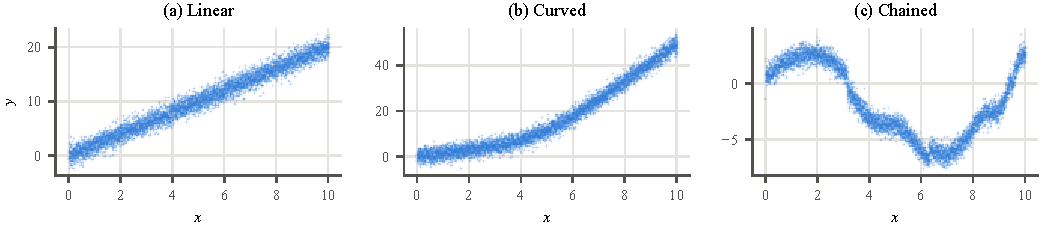
\includegraphics[width=\textwidth]{fig_tasks}
\caption{The three synthetic regression tasks ($N=5{,}000$). (a)~linear with $\sigma=1$; (b)~quadratic plus
sinusoid with $\sigma=2$; (c)~a three-stage composition containing a square-wave discontinuity, $\sigma=0.5$.}
\label{fig:tasks}
\end{figure*}
\fi

% Architecture schematics for the six parameter-matched models (Section III).
% FC n = fully connected layer with n outputs; R = ReLU. Edit freely in Overleaf.
\begin{figure*}[t]
\centering
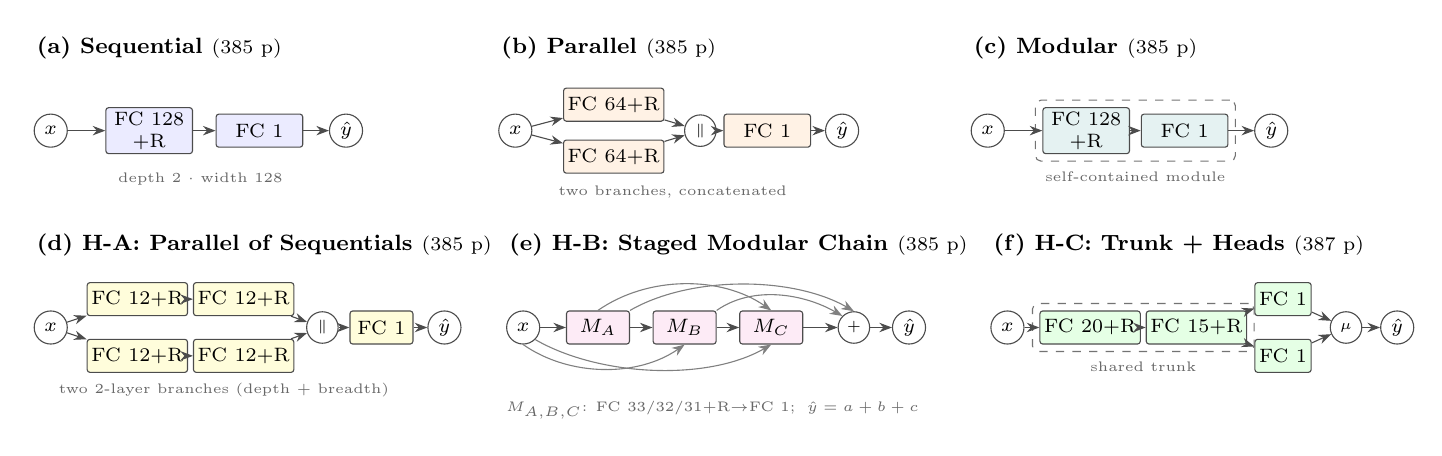
\begin{tikzpicture}[
  font=\scriptsize,
  >={Stealth[length=1.6mm]},
  io/.style={circle, draw=black!70, minimum size=4.2mm, inner sep=0pt},
  fc/.style={rectangle, rounded corners=1pt, draw=black!70, fill=#1, minimum height=4.2mm,
             minimum width=11mm, inner sep=1.5pt, align=center},
  fc/.default=blue!8,
  op/.style={circle, draw=black!70, fill=white, minimum size=4mm, inner sep=0pt},
  mod/.style={draw=black!55, dashed, rounded corners=2pt, inner sep=2.5pt},
  lab/.style={font=\footnotesize\bfseries, anchor=west},
  note/.style={font=\tiny, text=black!60},
  every edge/.style={draw=black!70, ->},
]
%------------------------------------------------ (a) Sequential
\begin{scope}[shift={(0,0)}]
  \node[lab] at (-0.3,1.05) {(a) Sequential \normalfont\scriptsize(385 p)};
  \node[io] (x) at (0,0) {$x$};
  \node[fc] (h) at (1.25,0) {FC 128\\+R};
  \node[fc] (o) at (2.65,0) {FC 1};
  \node[io] (y) at (3.75,0) {$\hat y$};
  \draw (x) edge (h) (h) edge (o) (o) edge (y);
  \node[note] at (1.9,-0.62) {depth 2 $\cdot$ width 128};
\end{scope}
%------------------------------------------------ (b) Parallel
\begin{scope}[shift={(5.9,0)}]
  \node[lab] at (-0.3,1.05) {(b) Parallel \normalfont\scriptsize(385 p)};
  \node[io] (x) at (0,0) {$x$};
  \node[fc=orange!10] (a) at (1.25,0.33) {FC 64+R};
  \node[fc=orange!10] (b) at (1.25,-0.33) {FC 64+R};
  \node[op] (c) at (2.35,0) {\tiny$\Vert$};
  \node[fc=orange!10] (o) at (3.2,0) {FC 1};
  \node[io] (y) at (4.15,0) {$\hat y$};
  \draw (x) edge (a) (x) edge (b) (a) edge (c) (b) edge (c) (c) edge (o) (o) edge (y);
  \node[note] at (2.0,-0.78) {two branches, concatenated};
\end{scope}
%------------------------------------------------ (c) Modular
\begin{scope}[shift={(11.9,0)}]
  \node[lab] at (-0.3,1.05) {(c) Modular \normalfont\scriptsize(385 p)};
  \node[io] (x) at (0,0) {$x$};
  \node[fc=teal!10] (h) at (1.25,0) {FC 128\\+R};
  \node[fc=teal!10] (o) at (2.5,0) {FC 1};
  \node[io] (y) at (3.6,0) {$\hat y$};
  \node[mod, fit=(h)(o), label={[note]below:self-contained module}] {};
  \draw (x) edge (h) (h) edge (o) (o) edge (y);
\end{scope}
%------------------------------------------------ (d) H-A
\begin{scope}[shift={(0,-2.5)}]
  \node[lab] at (-0.3,1.05) {(d) H-A: Parallel of Sequentials \normalfont\scriptsize(385 p)};
  \node[io] (x) at (0,0) {$x$};
  \node[fc=yellow!14] (a1) at (1.1,0.36) {FC 12+R};
  \node[fc=yellow!14] (a2) at (2.45,0.36) {FC 12+R};
  \node[fc=yellow!14] (b1) at (1.1,-0.36) {FC 12+R};
  \node[fc=yellow!14] (b2) at (2.45,-0.36) {FC 12+R};
  \node[op] (c) at (3.45,0) {\tiny$\Vert$};
  \node[fc=yellow!14, minimum width=8mm] (o) at (4.2,0) {FC 1};
  \node[io] (y) at (5.0,0) {$\hat y$};
  \draw (x) edge (a1) (a1) edge (a2) (x) edge (b1) (b1) edge (b2)
        (a2) edge (c) (b2) edge (c) (c) edge (o) (o) edge (y);
  \node[note] at (2.2,-0.8) {two 2-layer branches (depth + breadth)};
\end{scope}
%------------------------------------------------ (e) H-B
\begin{scope}[shift={(6.0,-2.5)}]
  \node[lab] at (-0.3,1.05) {(e) H-B: Staged Modular Chain \normalfont\scriptsize(385 p)};
  \node[io] (x) at (0,0) {$x$};
  \node[fc=magenta!8, minimum width=8mm] (A) at (0.95,0) {$M_A$};
  \node[fc=magenta!8, minimum width=8mm] (B) at (2.05,0) {$M_B$};
  \node[fc=magenta!8, minimum width=8mm] (C) at (3.15,0) {$M_C$};
  \node[op] (s) at (4.2,0) {\tiny$+$};
  \node[io] (y) at (4.9,0) {$\hat y$};
  \draw (x) edge (A) (A) edge (B) (B) edge (C) (C) edge (s) (s) edge (y);
  % outputs a, b also feed later stages and the sum (top); x skips to B and C (bottom)
  \draw[->, black!50] (A.north) to[out=35, in=145, looseness=0.9] (C.north);
  \draw[->, black!50] (A.north east) to[out=30, in=150, looseness=0.8] (s.north);
  \draw[->, black!50] (B.north east) to[out=35, in=150, looseness=0.9] (s.north west);
  \draw[->, black!50] (x.south) to[out=-35, in=-145, looseness=0.9] (B.south);
  \draw[->, black!50] (x.south east) to[out=-30, in=-150, looseness=0.8] (C.south);
  \node[note] at (2.4,-1.05) {$M_{A,B,C}$: FC 33/32/31+R$\rightarrow$FC 1;\; $\hat y = a+b+c$};
\end{scope}
%------------------------------------------------ (f) H-C
\begin{scope}[shift={(12.15,-2.5)}]
  \node[lab] at (-0.3,1.05) {(f) H-C: Trunk + Heads \normalfont\scriptsize(387 p)};
  \node[io] (x) at (0,0) {$x$};
  \node[fc=green!10] (t1) at (1.05,0) {FC 20+R};
  \node[fc=green!10] (t2) at (2.4,0) {FC 15+R};
  \node[fc=green!10, minimum width=7mm] (h1) at (3.5,0.36) {FC 1};
  \node[fc=green!10, minimum width=7mm] (h2) at (3.5,-0.36) {FC 1};
  \node[op] (m) at (4.3,0) {\tiny$\mu$};
  \node[io] (y) at (4.95,0) {$\hat y$};
  \node[mod, fit=(t1)(t2), label={[note]below:shared trunk}] {};
  \draw (x) edge (t1) (t1) edge (t2) (t2) edge (h1) (t2) edge (h2) (h1) edge (m) (h2) edge (m) (m) edge (y);
\end{scope}
\end{tikzpicture}
\caption{The six parameter-matched architectures (385 trainable parameters; 387 for \HC). Top row: the three
single-paradigm baselines from the pilot study. Bottom row: hybrids combining depth, breadth, and modularity.
FC~$n$ = fully connected layer with $n$ outputs, R = ReLU, $\Vert$ = concatenation, $\mu$ = mean.
Note that (a) and (c) compute the same function class; they differ only in how the code is organized,
which lets us use them as a control pair for implementation overhead (Section~\ref{sec:pilot}).}
\label{fig:arch}
\end{figure*}


\subsection{Architectures}
\label{sec:archs}
All six models (\cref{fig:arch}) are one-input, one-output multilayer models with ReLU
activations~\cite{nair2010rectified}, each with exactly 385 trainable parameters, so that differences in accuracy
or speed cannot be attributed to capacity. The one exception is \HC: no width pair for two-head wiring totals
385, so it uses the nearest configuration, 387 (+0.5\%). \Cref{tab:arch} lists their parameter counts,
multiply--accumulate operations (MACs) per sample, critical-path depth (linear layers between input and
output), tensor operations dispatched per forward call, and the low-level (ATen) kernels those operations execute.

\textbf{Single-paradigm baselines.} \emph{Sequential} is a 1--128--1 network. \emph{Parallel} feeds the input
to two 64-unit branches whose activations are concatenated before a linear read-out, in the spirit of
multi-branch designs such as Inception~\cite{szegedy2015going}. \emph{Modular} wraps a hidden layer and read-out
in a self-contained module. With 128 hidden units it calculates exactly the same function class as
Sequential, and under the same seed it initializes to the same weights. We keep it as a
\emph{control}: any measured difference between Sequential and Modular is implementation overhead or
timing noise, never architecture.

\textbf{Hybrids.} \textbf{\HA} (\emph{parallel of sequentials}) runs two 2-layer, 12-unit stacks side by side,
combining depth and breadth. \textbf{\HB} (\emph{staged modular chain}) has three sub-networks $M_A$, $M_B$, $M_C$ (hidden widths 33, 32,
and 31, chosen to total exactly 385 parameters) that mirror the three stages of the chained target: $M_B$ receives $(x,a)$, $M_C$ receives
$(x,a,b)$, and the output is $a+b+c$. This gives densely connected skip links in the spirit of
DenseNet~\cite{huang2017densenet} and an additive output similar to residual learning~\cite{he2016resnet}.
\textbf{\HC} (\emph{trunk + parallel heads}) shares a 2-layer trunk (20 and 15 units) between two linear heads whose
outputs are averaged, the hard-parameter-sharing pattern from multi-task learning~\cite{caruana1997multitask}.
No set of architectures can match parameters, MACs, and operation count at once. Fixing parameters forces the
other two to vary, and that difference is what lets us test which cost measure actually predicts latency.

\begin{table}[t]
\centering
\caption{Architecture cost profile. Depth: linear layers on the longest path. Ops / Kern.: PyTorch operations /
ATen kernels per forward call. Latency: median single-thread CPU time over 10 shuffled repeats; comp.: with
\texttt{torch.compile}.}
\label{tab:arch}
\setlength{\tabcolsep}{2.4pt}
\begin{tabular}{@{}lrrrrrrrr@{}}
\toprule
 & & \textbf{MACs/} & & & & \multicolumn{3}{c}{\textbf{Latency (\textmu s)}}\\
\cmidrule(l){7-9}
\textbf{Model} & \textbf{Params} & \textbf{sample} & \textbf{Depth} & \textbf{Ops} & \textbf{Kern.} & \textbf{b=1} & \textbf{comp.} & \textbf{4096}\\
\midrule
\tablebody{tables/tab_arch_body.tex}
\bottomrule
\end{tabular}
\end{table}

\subsection{Training Protocol}
Every model is implemented and trained in PyTorch~\cite{paszke2019pytorch} with one shared training loop. We use
Adam~\cite{kingma2015adam} (learning rate $10^{-3}$, $\beta=(0.9,0.999)$, $\epsilon=10^{-7}$, matching the Keras
default used in the pilot), mean-squared-error loss, mini-batches of 32 with per-epoch shuffling, and
100 epochs (12,500 optimizer steps). To test whether the chained-task results reflect undertraining, we also
train Sequential, Parallel, \HA, and \HB on the chained task for 300 epochs under the same protocol. Each (model, task) pair is trained with five seeds (0--4) that control
initialization and batch order. We report mean\,$\pm$\,standard deviation across seeds, following
recommendations to account for training variance in benchmark comparisons~\cite{bouthillier2021accounting}.

\subsection{Metrics}
\begin{itemize}
\item \textbf{Test MSE} and $R^2$ on the 1,000 held-out points after the final epoch.
\item \textbf{Convergence epoch}: the first epoch whose test MSE is within 5\% of that run's best.
\item \textbf{Training cost}: wall-clock training time divided by optimizer steps (ms/step).
\item \textbf{Inference latency}: median of 50 forward passes over the full test set (batch 1{,}000).
\end{itemize}
Significance against the Sequential baseline uses Welch's two-sample $t$-test on test MSE ($n=5$ per arm,
$p<0.05$).\ifcompact
 One timing group with a contention outlier was re-measured; accuracy was identical.
\else
 One timing group (\HB, chained task) was re-measured after a single seed's inference time deviated by
30\% from the same network on the other tasks; its accuracy was bit-identical across both passes.
\fi

\subsection{Latency Sweep}
\label{sec:sweep}
Real deployments rarely run inference at exactly the batch size used for evaluation, so we also time every
model at batch sizes $\{1, 8, 64, 512, 1000, 4096\}$ with 1 and 4 CPU threads. Each configuration
gets 50 warm-up calls followed by 1,000 timed calls, and the whole grid is repeated 10 times in a freshly shuffled
order so that run order and cache state cannot result in bias towards any model. We report the median of the per-repeat medians,
with a 95\% interval across repeats.
MACs are counted with forward hooks on every linear layer. Dispatched operations are counted by intercepting
PyTorch's \texttt{\_\_torch\_function\_\_} protocol during one forward pass, and the kernels those operations
execute are counted with \texttt{torch.profiler}. We also count \texttt{nn.Module} calls with forward
hooks. Finally, we time batch-1 inference after compiling each model with \texttt{torch.compile} (default
Inductor backend), using the same repeat protocol. These sweep timings are separate from the batch-1,000 inference
times in \cref{tab:main}, which are measured on the trained models inside the training study; the two agree where
they overlap.

\subsection{Environment}
All main-study and sweep measurements run on a single machine (Apple M5 CPU, macOS, Python~3.9,
PyTorch~\torchVersion) with \texttt{torch.set\_num\_threads(1)} unless stated otherwise, so the timings
compare architectures rather than thread scheduling. No GPU is used: at this model scale, kernel-launch
overhead would dominate any GPU measurement~\cite{sze2017efficient}. \ifanonymous All code and raw results will be released publicly upon
publication.\else All code and raw results are available at
\url{https://github.com/aryanamol10/Research-Paper-Comparative-Analysis-of-Neural-Models}.\fi

\section{Pilot Study: How a Benchmark Can Mislead}
\label{sec:pilot}

Before the main study, we ran a pilot benchmark (Benchmark~1) of the three single-paradigm models in a
Google Colab notebook. Its headline result was striking: the Modular network trained about
\pilotSpeedup$\times$ faster than Sequential and Parallel on every task\ifcompact\else\ (\cref{tab:pilot})\fi,
and its accuracy was only marginally worse. Taken at face value, this suggests that modularity is a free
latency win. Auditing the pilot showed that the result has nothing to do with architecture. We report the
audit because each flaw is common in small-scale benchmarking~\cite{lipton2019troubling,bouthillier2021accounting}.

\ifcompact\else  % dropped in the 6-page build
\begin{table}[t]
\centering
\caption{Pilot (Benchmark~1) results as originally reported: training time (s) and final \emph{training}
MSE, single seed. Compare the MSEs with the target variances: 34.7, 228.8, and 10.0.}
\label{tab:pilot}
\setlength{\tabcolsep}{3pt}
\begin{tabular}{@{}lrrrrrr@{}}
\toprule
 & \multicolumn{2}{c}{\textbf{Linear}} & \multicolumn{2}{c}{\textbf{Curved}} & \multicolumn{2}{c}{\textbf{Chained}}\\
\cmidrule(lr){2-3}\cmidrule(lr){4-5}\cmidrule(l){6-7}
\textbf{Model} & time & MSE & time & MSE & time & MSE\\
\midrule
\tablebody{tables/tab_pilot_body.tex}
\bottomrule
\end{tabular}
\end{table}
\fi

\textbf{Confound 1: framework, not architecture.} Sequential and Parallel were built in
Keras/TensorFlow~\cite{abadi2016tensorflow,chollet2015keras} using \texttt{model.fit}, while Modular was a
hand-written PyTorch loop. Modular and Sequential compute the same 1--128--1 function, so the
$\sim$11\,s gap is entirely framework and training-loop overhead. Framework-level differences of this size
are well documented~\cite{shi2016benchmarking}. They show that any timing comparison across frameworks
says little about architecture.

\textbf{Confound 2: uninformative inputs.} The pilot trained on $x\sim\mathcal U(0,1)$ drawn
independently of the targets, which were computed on the evenly spaced grid. With no information in the
inputs, the best any model can do is predict the target mean, which gives an MSE equal to the target variance.
The reported losses (37.8, 240, 10.4) sit just above those variances (34.7, 228.8, 10.0). In other words,
none of the pilot models learned the task, so their accuracy ranking is noise.

\textbf{Confound 3: no held-out data, one seed.} Losses were final-epoch \emph{training} losses from a single
seed with shuffling disabled, so neither generalization nor run-to-run variance could be assessed.

The main study (\cref{sec:method}) fixes all three: one framework and one training loop, true inputs, a held-out
split, and five seeds. The identical Sequential/Modular pair stays in as a built-in check. If the protocol is
sound, the two must agree on accuracy and differ only by noise.

\section{Results}
\label{sec:results}

\Cref{tab:main} reports accuracy and cost for every (model, task) pair, \cref{fig:curves} shows test-error
trajectories and behavior\ifcompact.\else, and \cref{fig:tradeoff} places each model on an accuracy-cost plane. \fi The latency sweep is shown in
\cref{fig:latency,fig:ops}.

\begin{table*}[t]
\centering
\caption{Main results (mean\,$\pm$\,std over 5 seeds; held-out test set of 1,000 points). Irreducible test MSE
is 1, 4, and 0.25 for the linear, curved, and chained tasks. Bold = best at shown precision.
$^\dagger$Welch's $t$-test vs.\ Sequential, $p<0.05$. Inference = forward pass over the whole test set
(batch 1,000), single CPU thread.}
\label{tab:main}
\begin{tabular}{@{}lccccc@{}}
\toprule
\textbf{Model} & \textbf{Test MSE} $\downarrow$ & $\boldsymbol{R^2}$ $\uparrow$ & \textbf{Train (ms/step)} $\downarrow$
& \textbf{Inference (ms)} $\downarrow$ & \textbf{Converge (epoch)} $\downarrow$\\
\midrule
\tablebody{tables/tab_main_body.tex}
\bottomrule
\end{tabular}
\end{table*}

\begin{figure*}[t]
\centering
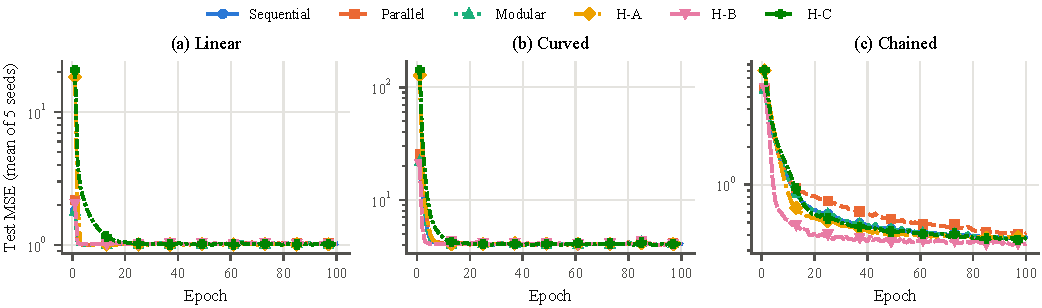
\includegraphics[width=\textwidth]{fig_curves}
\caption{Test MSE per epoch (log scale, mean of five seeds). Hybrids reach low error in far fewer epochs on the
curved and chained tasks. \HB (pink) is fastest to finish and ends lowest on the chained task.}
\label{fig:curves}
\end{figure*}

\subsection{The Control Pair: Identical Math, Different Code}
\label{sec:res-control}
Sequential and Modular compute the same function and, under the same seed, produce the same test MSE on every
task (\cref{tab:main}). Their training step times differ by only \ctrlStepGap\%, confirming that the pilot's
\pilotSpeedup$\times$ ``Modular advantage'' (\cref{sec:pilot}) disappears once the framework and training loop
are held constant. Their batch-1 inference latency, however, differs by \ctrlLatGap\% (\latOneSequential\ vs.\
\latOneModular\us), with non-overlapping 95\% intervals across ten shuffled repeats, so the gap is not run-order
noise. Both dispatch three tensor operations, but Sequential's \texttt{nn.Sequential} container makes
\modSequential\ \texttt{nn.Module} calls per forward pass against Modular's \modModular\ifcompact.\else. The control
pair therefore isolates a second, purely software overhead, telling us how the code organization costs time even when the
math is the same (\cref{sec:res-latency}).\fi

\subsection{Accuracy: Structure Pays Off Only When the Task Has Structure}
\label{sec:res-acc}
\textbf{Linear and curved tasks.} Every model reaches the noise floor on the linear task ($\text{MSE}\approx1$,
$R^2=0.971$), and on the curved task every model finishes within 2\% of the floor of 4. Simple targets
leave nothing for topology to improve upon, so at a 385-parameter budget the arrangement of parameters does not
change the final accuracy. It does change \emph{how fast} the floor is reached. On the curved task \HB converges in
\curvedConvHB\ epochs versus \curvedConvSeq\ for Sequential, about \curvedWallRatio$\times$ less
training time to convergence (\curvedWallHB\,s vs.\ \curvedWallSeq\,s) despite its higher cost per step.

\ifcompact\else  % dropped in the 6-page build
\textbf{Narrow trunks are fragile.} \HC's trunk width also matters for reliability. In a preliminary
configuration with a 17--17 trunk (376 parameters), one of five curved-task seeds settled in a poor solution
(MSE 21.4 vs.\ $\approx$4.0 for the rest). The exact-budget 20--15 trunk used here trains reliably on every
seed, but it still has the largest spread on the curved task.
\fi

\textbf{Chained task.} Here topology matters. \HB, in which the modules mirror the three stages of the target,
reaches \mseChainHB\ test MSE, \chainHBGain\% below Sequential (\mseChainSequential; $p<0.05$). \HA, which has no
knowledge of the stages, still improves by \chainHAGain\% (\mseChainHA; $p<0.05$). Measured against the noise floor
of 0.25, \HB's excess error (\chainExcessHB) is \chainExcessRatio$\times$ smaller than Sequential's
(\chainExcessSeq). Both hybrids also have much smaller variance ($\pm$0.02 vs.\ $\pm$0.12). The
single-paradigm models are still improving at epoch 100 (\cref{fig:curves}c), so part of their gap is slower
convergence rather than a lower ceiling. At a fixed budget, the gap is what a practitioner would get.
Plain breadth does not help: Parallel is the worst model on the chained task (\mseChainParallel).

\ifcompact\else  % dropped in the 6-page build
\begin{figure*}[t]
\centering
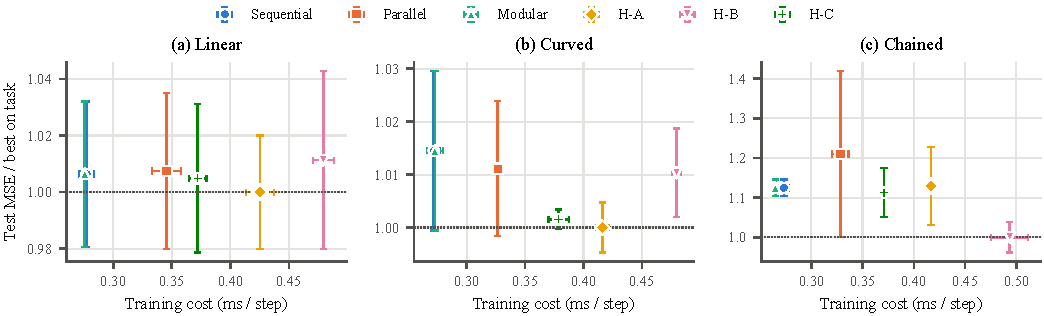
\includegraphics[width=\textwidth]{fig_tradeoff}
\caption{Accuracy vs.\ training cost. The $y$-axis is test MSE divided by the best model's MSE on that task (1 =
best). Error bars are $\pm$1 std over the seeds. On simple tasks all models tie on accuracy, so the cheapest
model wins. On the chained task, accuracy can be bought with per-step cost.}
\label{fig:tradeoff}
\end{figure*}
\fi

\subsection{Latency: Operator Count, Not Parameter Count}
\label{sec:res-latency}
\Cref{tab:arch} and \cref{fig:ops} show that, at a nearly constant parameter budget, single inference
latency spans almost 4$\times$, from \latOneModular\us (Modular) to \latOneHB\us (\HB). Parameter count
cannot explain this: all models have 385--387 parameters. Neither can MACs: Parallel and Sequential have the
same 256 MACs, but Parallel is slower, and \HC has the most MACs (350) but is faster than \HA and \HB. What does
explain it is the number of tensor operations dispatched per forward call. A linear fit of batch-1 latency on
operation count gives $R^2=\opsFitRsq$ with a slope of about \opsFitSlope\us per operation. At this scale, each
\texttt{Linear}, \texttt{ReLU}, \texttt{cat}, or add pays a constant framework transmission cost that lessens its
arithmetic. \HB has 13 operations and runs \latOneRatioHB$\times$ slower than Sequential. Counting the ATen
kernels those operations execute gives an equally good fit ($R^2=\kernFitRsq$), so the effect is not an artifact
of how we count.\ifcompact\ Adding \texttt{nn.Module} calls as a second predictor gives $R^2=\opsModFitRsq$ (descriptive only;
six points).\else Adding the number of \texttt{nn.Module} calls as a second predictor explains almost all
remaining variance ($R^2=\opsModFitRsq$; roughly \perOpUs\us per operation and \perModUs\us per module call),
including the Sequential/Modular gap. With six architectures and three fitted coefficients, we treat this
decomposition as being informative rather than predictive.\fi

\begin{figure}[t]
\centering
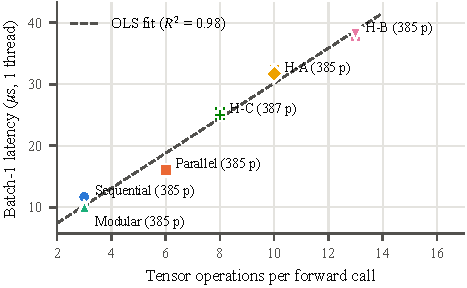
\includegraphics[width=\columnwidth]{fig_ops_latency}
\caption{Batch-1 inference latency vs.\ tensor operations per forward call. Parameter counts are in
parentheses; error bars are 95\% intervals across ten shuffled repeats. Latency is almost perfectly
explained by the operator count ($R^2=\opsFitRsq$) and is unrelated to the actual parameter count.}
\label{fig:ops}
\end{figure}

\ifcompact
\begin{figure}[t]
\centering
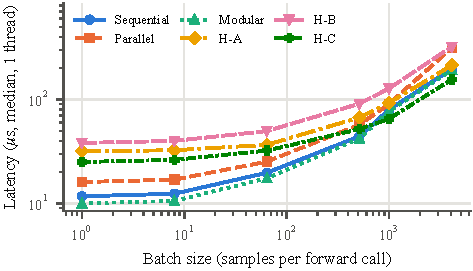
\includegraphics[width=\columnwidth]{fig_latency_batch_1t}
\caption{Inference latency vs.\ batch size (median over 10 shuffled repeats of 1,000 calls, one CPU thread). Curves are flat up to batch
$\approx$64, where overhead dominates and the ranking follows operator count. By batch 4096 the ranking
changes toward the narrow-activation \HC.}
\label{fig:latency}
\end{figure}
\else
\begin{figure*}[t]
\centering
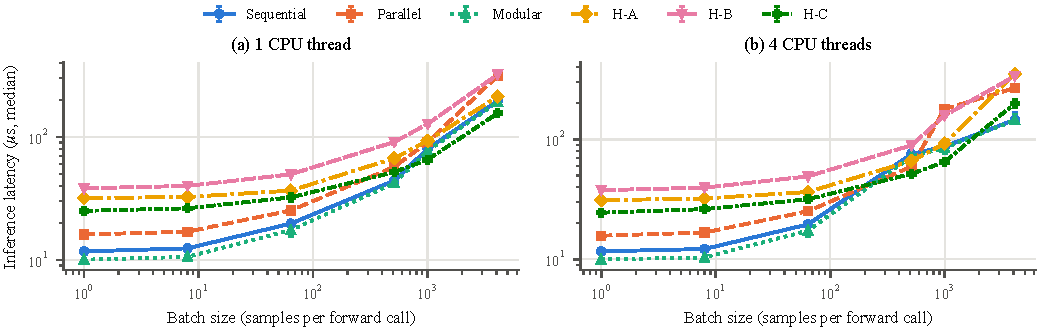
\includegraphics[width=\textwidth]{fig_latency_batch}
\caption{Inference latency vs.\ batch size (median over 10 shuffled repeats of 1,000 calls; bars show the
10th--90th percentile of individual calls). (a) With
one thread, the curves are flat up to batch $\approx$64, where overhead dominates, and the ranking follows
operator count. By batch 4096 it inverts toward the narrow-activation \HC. (b) Four threads rarely help models
this small and sometimes hurt (Parallel at batch 1,000).}
\label{fig:latency}
\end{figure*}
\fi

\textbf{Batch size changes the ranking.} \Cref{fig:latency}\ifcompact\else a\fi\ shows two regimes. Up to a batch of about 64,
latency is nearly flat and ordered by operator count. Past roughly 500 samples, per-element work takes over
and the ordering reshuffles. At batch 4096, \HC becomes the \emph{fastest} model (\latBigHC\us vs.\
\latBigSequential\us for Sequential) despite having the most MACs. This is consistent with memory traffic
having more value than arithmetic: \HC's widest activation is 20 values per sample, while Sequential's is 128 and
Parallel's concatenation writes 128 more. The two models that build intermediate concatenated tensors are the
slowest at batch 4096: \HB (\latBigHB\us) and Parallel (\latBigParallel\us). The latency ranking of these architectures, for this reason, depends on the batch size at of which it
is being measured.

\ifcompact\else  % dropped in the 6-page build (4-thread panel not shown)
\textbf{Threads.} With four occuring threads\ifcompact\else\ (\cref{fig:latency}b)\fi, batch-1 latency is unchanged. At larger batches the
effect is not the same. Sequential improves at batch 4096 (\latBigSequential\ to \threadSeqBigFour\us), but
Parallel at batch 1,000 slows from \threadParallelOne\ to \threadParallelFour\us and \HA at batch 4096 slows to
\threadHABigFour\us. For below kilobyte models, thread synchronization overhead can go over the parallel work.
\fi

\section{Discussion}
\label{sec:discussion}

\subsection{Which Architecture Should a Practitioner Pick?}
The results support a simple decision rule for small models on latency-sensitive paths.
\begin{enumerate}
\item \emph{If the target has no known structure, keep it shallow and minimize operators.} On the linear and
curved tasks every topology reached the noise floor, so the cheapest one, a single wide hidden layer with three
operations, becomes the best choice. It trains fastest per step and has the lowest batch-1 latency.
\item \emph{If the target is compositional and its stages are known, a staged modular hybrid is worth its
overhead.} \HB cut chained-task excess error by \chainExcessRatio$\times$ at \stepRatioHB$\times$ the training cost per
step and \latOneRatioHB$\times$ the batch-1 latency. For offline or batched inference, that trade is
attractive. For per-sample loops, this is not the case.
\item \emph{Measure latency at the deployment batch size.} The ranking at batch 1 (operator-bound) and at batch
4096 (memory-bound) differ. A benchmark at one batch size can recommend the incorrect model for another.
\end{enumerate}

\ifcompact\else  % dropped in the 6-page build (summarized in Section V-B)
\subsection{Hybrids Converge Faster}
A less expected result is how much faster the hybrids converge. \HB reached the curved-task noise floor in
\curvedConvHB\ epochs, and \HA in 24, against \curvedConvSeq\ for single models. We hypothesize that the
additive multi-path output acts like a remaining groupage ~\cite{he2016resnet,lakshminarayanan2017simple}, where several
sub-networks fit different parts of the target at once, so no single narrow path is required to carry the whole
function. When training compute rather than inference latency is the bottleneck, this can outweigh the hybrids'
higher per-step cost.
\fi

\ifcompact\else  % dropped in the 6-page build (overlaps Section IV)
\subsection{Lessons for Small-Scale Benchmarking}
The pilot study shows how easily a benchmark can produce a confident, wrong
conclusion. Three practices caught it and are cheap enough for any student or practitioner to conduct. First,
include a \emph{null control}: a pair that should show no difference, such as our identical Sequential and
Modular networks. Our benchmarking served multiple roles, exposing the pilot's framework confound, catching CPU contention during
one training pass, and revealing module-call overhead that operation counts alone miss. Second, hold the framework and training loop fixed so that timing measures the model and not
the software stack~\cite{shi2016benchmarking}. Third, check accuracy against small baselines. A model's output that gives
the loss being equal to the target variance has not learned anything~\cite{lipton2019troubling}.
\fi

\subsection{Limitations and Threats to Validity}
\textbf{Scale.} The models are tiny ($\approx$385 parameters) and the tasks shown for testing are one-dimensional. This is
done deliberately, as it isolates the topology from overall capacity and makes the five-seed run cheap. It also means the
total latencies are dominated by per-operator overhead in a way that will shrink, though not vanish, for larger
models, where compute and traffic take over~\cite{sze2017efficient}. The ranking of architectures at
batch~4096, where arithmetic begins to matter, is a better guide to larger-scale behavior than batch~1.

\textbf{Hardware and runtime.} All timings come from one Apple M5 CPU running eager-mode PyTorch. Graph
compilers (TorchScript, \texttt{torch.compile}, ONNX Runtime) fuse small operators and would likely create narrowing in the
count penalty we observe. GPUs and microcontrollers would have very different overhead profiles. We
therefore present latency \emph{trends} across architectures, not total numbers to be quoted for other
platforms.\todo{optional: rerun latency\_sweep.py with torch.compile or on a Raspberry Pi / Colab GPU for a
second hardware point}

\textbf{Task design.} The chained task was written by the same author who designed \HB, so \HB's structural
match to it is an intentional best case for modular inductive bias, not an unbiased test. We do not claim
that staged modularity helps on unknown compositional problems, only that it \emph{can} when the
decomposition is known.

\textbf{Statistics.} Five seeds detect large effects but not small ones. We report Welch's $t$-tests
without multiple-comparison correction, so single and marginal results should be read as suggestive.
Hyperparameters (learning rate, epochs, batch size) were fixed for all models rather than tuned per
architecture, which may disadvantage architectures that give preference for other settings.

\section{Conclusion}
\label{sec:conclusion}

We benchmarked six neural architectures that share a 385-parameter budget and differ only in how those parameters
are arranged. Three findings stand out. First, configuration changes final accuracy only when the target has
structure for it to match. A staged modular hybrid reduced error on a compositional task by \chainHBGain\%, a gap that
held after 300 epochs, while every other structure tied on simple tasks. Second, small-model latency is decided by
operator count at small batch sizes and by activation width at large ones, and parameter count predicts neither;
\texttt{torch.compile} narrows the operator-count penalty but adds a fixed per-call cost. Third, protocol choices can
masquerade as architecture effects: a cross-framework confound in our pilot and unscaled targets in an earlier run
both produced large apparent advantages that disappeared under a controlled protocol.

Future work will extend the study to other runtimes (ONNX Runtime) and hardware (GPUs, neural accelerators,
microcontrollers), to larger parameter budgets where arithmetic dominates overhead, and to real-world tasks where
the stage decomposition must be learned rather than designed.


% Contains no identifying information, so it is kept in the double-blind build as well.
\section*{Acknowledgment}
The pilot study used Google Colab. AI tools assisted with experiment code, figures, and drafting;
\ifanonymous the authors\else the author\fi\ verified all content.

\bibliographystyle{IEEEtran}
\bibliography{references}

\end{document}
